% ĐỢT 7: CỤM 5 (ĐỀ 1 & ĐỀ 2) - BỘ ĐỀ THAM KHẢO TUYỂN SINH 10 NĂM HỌC 2026-2027 SỞ GD&ĐT TP.HCM

% ==============================================================================
% CỤM 5 - ĐỀ THAM KHẢO 1 (Trang 27-28, Đề số 13)
% ==============================================================================

\begin{bt}%[9D6H18-2]
% nguon: Đề tham khảo Tuyển sinh 10 năm học 2026-2027 Sở GD&ĐT TP.HCM - Cụm 5 Đề 1 - Bài 1
Cho hàm số $y = 2x^2$ có đồ thị $(P)$.
\begin{enumerate}[a)]
	\item Vẽ đồ thị $(P)$ trên hệ trục tọa độ $Oxy$.
	\item Tìm tọa độ các điểm thuộc $(P)$ có tung độ bằng $16$.
\end{enumerate}
\loigiai{
\begin{enumerate}[a)]
	\item Bảng giá trị của hàm số $y = 2x^2$:
	\begin{center}
		\begin{tabular}{|c|c|c|c|c|c|}
			\hline
			$x$ & $-2$ & $-1$ & $0$ & $1$ & $2$ \\ \hline
			$y$ & $8$ & $2$ & $0$ & $2$ & $8$ \\ \hline
		\end{tabular}
	\end{center}
	Đồ thị $(P)$ là một parabol đi qua các điểm $(-2; 8)$, $(-1; 2)$, $(0; 0)$, $(1; 2)$, $(2; 8)$, nhận trục tung $Oy$ làm trục đối xứng và có đỉnh là gốc tọa độ $O(0;0)$.
	\begin{center}
		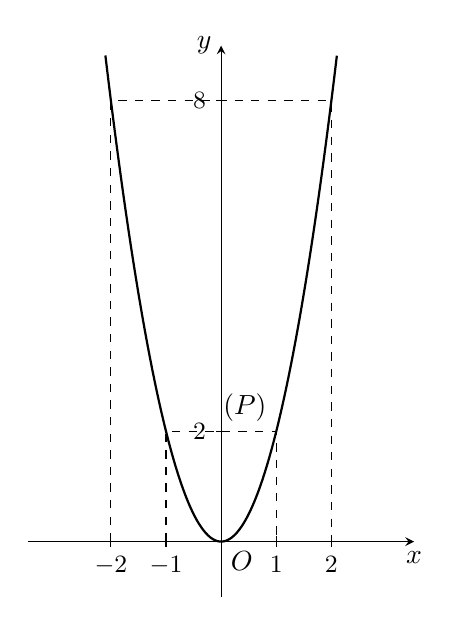
\begin{tikzpicture}[>=stealth,scale=0.7]
			\draw[->] (-3.5,0) -- (3.5,0) node[below] {$x$};
			\draw[->] (0,-1) -- (0,9) node[left] {$y$};
			\draw (0,0) node[below right] {$O$};
			\foreach \x in {-2,-1,1,2}
				\draw (\x,0.1) -- (\x,-0.1) node[below] {\small $\x$};
			\foreach \y in {2,8}
				\draw (0.1,\y) -- (-0.1,\y) node[left] {\small $\y$};
			\draw[dashed] (-1,0) -- (-1,2) -- (1,2) -- (1,0);
			\draw[dashed] (-2,0) -- (-2,8) -- (2,8) -- (2,0);
			\draw[thick,smooth,samples=100,domain=-2.1:2.1] plot(\x,{2*(\x)^2});
			\node[above left] at (1,2) {$(P)$};
		\end{tikzpicture}
	\end{center}
	\item Gọi điểm cần tìm là $N(x; y)$. Vì điểm $N$ thuộc $(P)$ và có tung độ bằng $16$ nên:
	$$2x^2 = 16 \iff x^2 = 8 \iff x = \pm 2\sqrt{2}.$$
	Vậy có hai điểm thỏa mãn yêu cầu là $(2\sqrt{2}; 16)$ và $(-2\sqrt{2}; 16)$.
\end{enumerate}
}
\end{bt}

\begin{bt}%[9D6H20-2]
% nguon: Đề tham khảo Tuyển sinh 10 năm học 2026-2027 Sở GD&ĐT TP.HCM - Cụm 5 Đề 1 - Bài 2
Cho phương trình bậc hai $-x^2 + 10x + 8 = 0$.
\begin{enumerate}[a)]
	\item Chứng minh phương trình trên luôn có hai nghiệm phân biệt $x_1, x_2$.
	\item Không giải phương trình, hãy tính giá trị của biểu thức:
	$$A = (x_1 - x_2)(x_1^2 - x_2^2).$$
\end{enumerate}
\loigiai{
\begin{enumerate}[a)]
	\item Phương trình $-x^2 + 10x + 8 = 0$ có các hệ số $a = -1$, $b = 10$, $c = 8$.\\
	Ta có:
	$$\Delta = b^2 - 4ac = 10^2 - 4 \cdot (-1) \cdot 8 = 100 + 32 = 132 > 0.$$
	Vì $\Delta > 0$ nên phương trình luôn có hai nghiệm phân biệt $x_1, x_2$.
	\item Theo định lí Vi-ét, ta có:
	$$\left\{\begin{aligned} &x_1 + x_2 = -\dfrac{b}{a} = -\dfrac{10}{-1} = 10 \\ &x_1 x_2 = \dfrac{c}{a} = \dfrac{8}{-1} = -8. \end{aligned}\right.$$
	Ta có:
	$$x_1^2 + x_2^2 = (x_1 + x_2)^2 - 2x_1 x_2 = 10^2 - 2 \cdot (-8) = 100 + 16 = 116.$$
	Biến đổi biểu thức $A$:
	\begin{align*}
		A &= (x_1 - x_2)(x_1^2 - x_2^2) = (x_1 - x_2)(x_1 - x_2)(x_1 + x_2) \\
		&= (x_1 - x_2)^2(x_1 + x_2) \\
		&= (x_1^2 - 2x_1 x_2 + x_2^2)(x_1 + x_2) \\
		&= (x_1^2 + x_2^2 - 2x_1 x_2)(x_1 + x_2).
	\end{align*}
	Thay các giá trị Vi-ét vào, ta được:
	$$A = \big(116 - 2 \cdot (-8)\big) \cdot 10 = (116 + 16) \cdot 10 = 132 \cdot 10 = 1320.$$
	Vậy $A = 1320$.
\end{enumerate}
}
\end{bt}

\begin{bt}%[9D8H26-3]
% nguon: Đề tham khảo Tuyển sinh 10 năm học 2026-2027 Sở GD&ĐT TP.HCM - Cụm 5 Đề 1 - Bài 3
Biểu đồ hình quạt tròn biểu diễn kết quả thống kê chọn môn thể thao yêu thích nhất của $440$ học sinh khối 9 ở một trường trung học cơ sở: Cầu lông ($25\%$), Bóng đá ($35\%$), Bóng bàn ($15\%$), Bóng chuyền ($25\%$). Mỗi học sinh chỉ chọn đúng một môn thể thao.
\begin{enumerate}[a)]
	\item Tính số lượng học sinh cụ thể yêu thích mỗi môn thể thao.
	\item Chọn ngẫu nhiên một bạn học sinh khối 9. Tính xác suất để bạn được chọn không thích môn Cầu lông.
\end{enumerate}
\loigiai{
\begin{enumerate}[a)]
	\item Số lượng học sinh yêu thích từng môn thể thao là:
	\begin{itemize}
		\item Môn Cầu lông: $440 \cdot 25\% = 110$ (học sinh).
		\item Môn Bóng đá: $440 \cdot 35\% = 154$ (học sinh).
		\item Môn Bóng bàn: $440 \cdot 15\% = 66$ (học sinh).
		\item Môn Bóng chuyền: $440 \cdot 25\% = 110$ (học sinh).
	\end{itemize}
	\item Không gian mẫu có số phần tử là $n(\Omega) = 440$.\\
	Gọi $E$ là biến cố: ``Học sinh được chọn không thích môn Cầu lông''.\\
	Số học sinh không thích môn Cầu lông là:
	$$n(E) = 154 + 66 + 110 = 330\text{ (học sinh)}.$$
	Xác suất của biến cố $E$ là:
	$$P(E) = \dfrac{n(E)}{n(\Omega)} = \dfrac{330}{440} = \dfrac{3}{4}.$$
\end{enumerate}
}
\end{bt}

\begin{bt}%[9D6V21-3]
% nguon: Đề tham khảo Tuyển sinh 10 năm học 2026-2027 Sở GD&ĐT TP.HCM - Cụm 5 Đề 1 - Bài 4
Một vườn hoa hình chữ nhật có chiều dài $20\text{ m}$ và chiều rộng $14\text{ m}$. Người ta làm một lối đi ngang sát cạnh trên và một lối đi dọc ở giữa khu vườn với cùng bề rộng là $x$ mét ($0 < x < 14$). Phần đất còn lại dùng để trồng hoa.
\begin{enumerate}[a)]
	\item Viết biểu thức $S$ biểu diễn theo $x$ diện tích phần đất trồng hoa.
	\item Tìm bề rộng $x$ của lối đi, biết rằng diện tích đất trồng hoa bằng $187\text{ m}^2$.
\end{enumerate}
\loigiai{
\begin{enumerate}[a)]
	\item Lối đi dọc có bề rộng là $x$ mét, nên chiều dài phần đất trồng hoa còn lại là $20 - x\text{ (m)}$.\\
	Lối đi ngang sát cạnh trên có bề rộng là $x$ mét, nên chiều rộng phần đất trồng hoa còn lại là $14 - x\text{ (m)}$.\\
	Biểu thức diện tích phần đất dùng để trồng hoa là:
	$$S = (20 - x)(14 - x)\text{ (m}^2\text{)}.$$
	\item Vì diện tích đất trồng hoa bằng $187\text{ m}^2$, ta có phương trình:
	$$(20 - x)(14 - x) = 187 \iff x^2 - 34x + 280 = 187 \iff x^2 - 34x + 93 = 0.$$
	Phương trình có biệt thức $\Delta' = (-17)^2 - 1 \cdot 93 = 289 - 93 = 196 = 14^2 > 0$.\\
	Nghiệm của phương trình:
	$$\left[\begin{aligned} &x_1 = 17 - 14 = 3\text{ (thỏa mãn } 0 < x < 14\text{)} \\ &x_2 = 17 + 14 = 31\text{ (loại vì } x > 14\text{)}. \end{aligned}\right.$$
	Vậy bề rộng của lối đi là $3\text{ m}$.
\end{enumerate}
}
\end{bt}

\begin{bt}%[9H0V31-3]
% nguon: Đề tham khảo Tuyển sinh 10 năm học 2026-2027 Sở GD&ĐT TP.HCM - Cụm 5 Đề 1 - Bài 5
Quan sát trên quả địa cầu thấy vị trí nước Việt Nam trải dài trên cung kinh tuyến từ vĩ độ $23^\circ 23'$ Bắc đến $8^\circ 27'$ Bắc theo hướng Bắc -- Nam và có chiều dài khoảng $1655\text{ km}$. Giả sử Trái Đất là hình cầu và có diện tích bề mặt được cho bởi công thức $S = 4\pi R^2$ (trong đó $S$ là diện tích, $R$ là bán kính mặt cầu; lấy $\pi \approx 3{,}14$).
\begin{enumerate}[a)]
	\item Hãy tính độ dài đường kinh tuyến và bán kính Trái Đất (làm tròn các kết quả đến hàng trăm kilômét).
	\item Biết diện tích rừng chiếm $20\%$ diện tích bề mặt Trái Đất, trong đó có $10\%$ là diện tích rừng nhiệt đới. Tính diện tích rừng nhiệt đới trên Trái Đất (làm tròn kết quả đến hàng trăm kilômét vuông).
\end{enumerate}
\loigiai{
\begin{enumerate}[a)]
	\item Số đo cung kinh tuyến tương ứng với vị trí nước Việt Nam là:
	$$\alpha = 23^\circ 23' - 8^\circ 27' = 14^\circ 56' = \left(14 + \dfrac{56}{60}\right)^\circ = \left(\dfrac{224}{15}\right)^\circ.$$
	Độ dài đường kinh tuyến (nửa chu vi hình tròn lớn của Trái Đất, ứng với $180^\circ$) là:
	$$L = \dfrac{1655 \cdot 180}{\dfrac{224}{15}} = \dfrac{4\,468\,500}{224} \approx 19\,948{,}66\text{ (km)}.$$
	Làm tròn đến hàng trăm là $20\,000\text{ km}$.\\
	Bán kính Trái Đất là:
	$$R = \dfrac{L}{\pi} = \dfrac{4\,468\,500}{224 \cdot 3{,}14} \approx 6\,353{,}08\text{ (km)}.$$
	Làm tròn đến hàng trăm là $6\,400\text{ km}$.
	\item Diện tích toàn bộ bề mặt Trái Đất là:
	$$S = 4\pi R^2 = 4 \cdot 3{,}14 \cdot \left(\dfrac{4\,468\,500}{224 \cdot 3{,}14}\right)^2 \approx 506\,915\,700\text{ (km}^2\text{)}.$$
	Diện tích rừng nhiệt đới chiếm tỉ lệ: $20\% \cdot 10\% = 2\% = 0{,}02$ diện tích bề mặt Trái Đất.\\
	Diện tích rừng nhiệt đới trên Trái Đất là:
	$$S_{\text{rnt}} = 0{,}02 \cdot S \approx 0{,}02 \cdot 506\,915\,700 \approx 10\,138\,300\text{ (km}^2\text{)}$$
	(hoặc tính theo $R = 6400\text{ km}$ thì $S_{\text{rnt}} = 0{,}02 \cdot 4 \cdot 3{,}14 \cdot 6400^2 \approx 10\,289\,200\text{ km}^2$, theo đáp án Sở là khoảng $10\,281\,500\text{ km}^2$).
\end{enumerate}
}
\end{bt}

\begin{bt}%[9D1H3-4]
% nguon: Đề tham khảo Tuyển sinh 10 năm học 2026-2027 Sở GD&ĐT TP.HCM - Cụm 5 Đề 1 - Bài 6
Hai cây nến có chiều dài ban đầu bằng nhau nhưng làm bằng chất liệu khác nhau. Cây nến thứ nhất cháy hết trong $3$ giờ, cây nến thứ hai cháy hết trong $4$ giờ. Người ta đốt hai cây nến cùng một lúc. Hỏi sau bao lâu thì chiều dài phần còn lại của cây nến thứ hai gấp đôi chiều dài phần còn lại của cây nến thứ nhất?
\loigiai{
Gọi $x$ (giờ) là thời gian cháy từ lúc bắt đầu đốt đến khi chiều dài phần còn lại của cây thứ hai gấp đôi cây thứ nhất ($0 < x < 3$).\\
Gọi chiều dài ban đầu của mỗi cây nến là $1$ (đơn vị độ dài).\\
Trong $1$ giờ:
\begin{itemize}
	\item Cây nến thứ nhất cháy được $\dfrac{1}{3}$ cây nến.
	\item Cây nến thứ hai cháy được $\dfrac{1}{4}$ cây nến.
\end{itemize}
Sau $x$ giờ:
\begin{itemize}
	\item Chiều dài phần còn lại của cây nến thứ nhất là $1 - \dfrac{x}{3}$.
	\item Chiều dài phần còn lại của cây nến thứ hai là $1 - \dfrac{x}{4}$.
\end{itemize}
Theo đề bài, chiều dài phần còn lại của cây nến thứ hai gấp đôi cây nến thứ nhất, ta có phương trình:
$$1 - \dfrac{x}{4} = 2\left(1 - \dfrac{x}{3}\right) \iff 1 - \dfrac{x}{4} = 2 - \dfrac{2x}{3} \iff \dfrac{2x}{3} - \dfrac{x}{4} = 2 - 1 \iff \dfrac{5x}{12} = 1 \iff x = \dfrac{12}{5} = 2{,}4\text{ (giờ)}.$$
Đổi: $2{,}4\text{ giờ} = 2\text{ giờ } 24\text{ phút}$.\\
Vậy sau $2{,}4$ giờ (tức $2$ giờ $24$ phút) thì chiều dài phần còn lại của cây nến thứ hai gấp đôi cây thứ nhất.
}
\end{bt}

\begin{bt}%[9H9C29-3]
% nguon: Đề tham khảo Tuyển sinh 10 năm học 2026-2027 Sở GD&ĐT TP.HCM - Cụm 5 Đề 1 - Bài 7
Cho đường tròn $(O; R)$ có hai đường kính $AB$ và $CD$ vuông góc với nhau tại $O$. Gọi $I$ là trung điểm của bán kính $OB$. Tia $CI$ cắt đường tròn $(O)$ tại điểm $E$ ($E$ khác $C$). Gọi $H$ là giao điểm của $AE$ và $CD$.
\begin{enumerate}[a)]
	\item Chứng minh bốn điểm $O, I, E, D$ cùng thuộc một đường tròn và $CO \cdot CD = CI \cdot CE$.
	\item Chứng minh $AH \cdot AE = 2R^2$ và $OA = 3 \cdot OH$.
	\item Gọi $K$ là hình chiếu của $O$ trên đoạn thẳng $BD$, $Q$ là giao điểm của $AD$ và $BE$. Chứng minh ba điểm $Q, K, I$ thẳng hàng.
\end{enumerate}
\loigiai{
\begin{center}
	\begin{tikzpicture}[scale=0.9,>=stealth]
		\coordinate (O) at (0,0);
		\def\R{2.8}
		\draw[thick] (O) circle (\R);
		\coordinate (A) at (-\R,0);
		\coordinate (B) at (\R,0);
		\coordinate (C) at (0,\R);
		\coordinate (D) at (0,-\R);
		\coordinate (I) at ($(O)!0.5!(B)$);
		% E la giao diem cua CI va (O)
		% Toa do I(1.4, 0), C(0, 2.8)
		% Vector CI: (1.4, -2.8). Phuong trinh duong thang CI: y - 2.8 = -2x => y = -2x + 2.8
		% x^2 + (-2x + 2.8)^2 = R^2 = 7.84 => 5x^2 - 11.2x = 0 => x = 11.2 / 5 = 2.24
		\coordinate (E) at (2.24, -1.68);
		\coordinate (H) at (intersection of A--E and C--D);
		\coordinate (K) at ($(B)!(O)!(D)$);
		\coordinate (Q) at (intersection of A--D and B--E);

		\draw[thick] (A) -- (B);
		\draw[thick] (C) -- (D);
		\draw[thick] (C) -- (E);
		\draw[thick] (A) -- (E);
		\draw[thick] (A) -- (Q);
		\draw[thick] (B) -- (Q);
		\draw[thick] (B) -- (D);
		\draw[thick] (O) -- (K);
		\draw[dashed] (E) -- (D);
		\draw[dashed] (Q) -- (I);

		\fill (O) circle (1.5pt) node[below left] {$O$};
		\fill (A) circle (1.5pt) node[left] {$A$};
		\fill (B) circle (1.5pt) node[right] {$B$};
		\fill (C) circle (1.5pt) node[above] {$C$};
		\fill (D) circle (1.5pt) node[below] {$D$};
		\fill (I) circle (1.5pt) node[above] {$I$};
		\fill (E) circle (1.5pt) node[below right] {$E$};
		\fill (H) circle (1.5pt) node[above left] {$H$};
		\fill (K) circle (1.5pt) node[above right] {$K$};
		\fill (Q) circle (1.5pt) node[below left] {$Q$};
	\end{tikzpicture}
\end{center}
\begin{enumerate}[a)]
	\item Vì $AB \perp CD$ tại $O$ nên tam giác $IOD$ vuông tại $O$, do đó $O$ thuộc đường tròn đường kính $ID$.\\
	Ta có $\widehat{CED} = 90^\circ$ (góc nội tiếp chắn nửa đường tròn đường kính $CD$), nên tam giác $IED$ vuông tại $E$, do đó $E$ thuộc đường tròn đường kính $ID$.\\
	Vậy bốn điểm $O, I, E, D$ cùng thuộc đường tròn đường kính $ID$.\\
	Xét $\Delta COI$ và $\Delta CED$ có:
	\begin{itemize}
		\item Góc $\widehat{OCE}$ chung;
		\item $\widehat{COI} = \widehat{CED} = 90^\circ$.
	\end{itemize}
	Do đó $\Delta COI \backsim \Delta CED$ (g-g) $\implies \dfrac{CO}{CE} = \dfrac{CI}{CD} \implies CO \cdot CD = CI \cdot CE$.
	\item Ta có $\widehat{AEB} = 90^\circ$ (góc nội tiếp chắn nửa đường tròn đường kính $AB$).\\
	Xét $\Delta AOH$ và $\Delta AEB$ có:
	\begin{itemize}
		\item Góc $\widehat{EAB}$ chung;
		\item $\widehat{AOH} = \widehat{AEB} = 90^\circ$.
	\end{itemize}
	Do đó $\Delta AOH \backsim \Delta AEB$ (g-g) $\implies \dfrac{AO}{AE} = \dfrac{AH}{AB} \implies AH \cdot AE = AO \cdot AB$.\\
	Vì $AO = R$ và $AB = 2R$ nên:
	$$AH \cdot AE = R \cdot 2R = 2R^2.$$
	Vì $I$ là trung điểm của $OB$ nên $IB = \dfrac{R}{2}$, do đó $IA = AB - IB = 2R - \dfrac{R}{2} = \dfrac{3R}{2}$.\\
	Suy ra $\dfrac{IA}{IB} = \dfrac{\dfrac{3R}{2}}{\dfrac{R}{2}} = 3$ (1).\\
	Mặt khác, tam giác $OCD$ vuông cân tại $O$ ($OC = OD = R$) nên $\widehat{CDB} = 45^\circ$.\\
	Suy ra $\widehat{CEB} = \widehat{CDB} = 45^\circ$ (cùng chắn cung $CB$).\\
	Vì $\widehat{AEB} = 90^\circ$ nên $\widehat{AEI} = 90^\circ - \widehat{IEB} = 90^\circ - 45^\circ = 45^\circ$.\\
	Suy ra $\widehat{AEI} = \widehat{IEB} = 45^\circ$, tức là $EI$ là tia phân giác của góc $\widehat{AEB}$ trong $\Delta AEB$.\\
	Áp dụng tính chất đường phân giác:
	$$\dfrac{EA}{EB} = \dfrac{IA}{IB} = 3\text{ (theo (1))}.$$
	Từ $\Delta AOH \backsim \Delta AEB$, ta có $\dfrac{OA}{OH} = \dfrac{AE}{EB} = 3 \implies OA = 3 \cdot OH$.
	\item Tam giác $ABD$ có $DO$ là đường trung tuyến ứng với cạnh $AB$. Vì $OA = OD = R$ nên $OD = 3 \cdot OH \implies OH = \dfrac{1}{3}OD$, suy ra $H$ là trọng tâm của tam giác $ABD$.\\
	Tam giác $OBD$ cân tại $O$ ($OB = OD = R$) có đường cao $OK$, nên $OK$ cũng là đường trung tuyến, suy ra $K$ là trung điểm của $BD$.\\
	Do đó $AK$ là đường trung tuyến của tam giác $ABD$, nên đường trung tuyến $AK$ phải đi qua trọng tâm $H$.\\
	Mà $A, E, H$ thẳng hàng nên bốn điểm $A, H, E, K$ thẳng hàng.\\
	Trong tam giác $QAB$, hai đường cao $BD$ và $AE$ (tức $AK$) cắt nhau tại $K$, nên $K$ là trực tâm của tam giác $QAB$.\\
	Suy ra $QK \perp AB$ (3).\\
	Mặt khác, xét tam giác $OBD$ có $I$ là trung điểm $OB$ và $K$ là trung điểm $BD$, nên $IK$ là đường trung bình của tam giác $OBD$.\\
	Suy ra $IK \parallel OD$. Mà $OD \perp AB$ tại $O$, nên $IK \perp AB$ (4).\\
	Từ (3) và (4), suy ra ba điểm $Q, K, I$ thẳng hàng.
\end{enumerate}
}
\end{bt}


% ==============================================================================
% CỤM 5 - ĐỀ THAM KHẢO 2 (Trang 29-30, Đề số 14)
% ==============================================================================

\begin{bt}%[9D6H18-2]
% nguon: Đề tham khảo Tuyển sinh 10 năm học 2026-2027 Sở GD&ĐT TP.HCM - Cụm 5 Đề 2 - Bài 1
Cho hàm số $y = x^2$ có đồ thị là Parabol $(P)$.
\begin{enumerate}[a)]
	\item Vẽ đồ thị $(P)$ của hàm số trên mặt phẳng tọa độ $Oxy$.
	\item Tìm tọa độ những điểm $M$ thuộc $(P)$ có tung độ bằng hai lần hoành độ bằng phép tính.
\end{enumerate}
\loigiai{
\begin{enumerate}[a)]
	\item Bảng giá trị của hàm số $y = x^2$:
	\begin{center}
		\begin{tabular}{|c|c|c|c|c|c|}
			\hline
			$x$ & $-2$ & $-1$ & $0$ & $1$ & $2$ \\ \hline
			$y$ & $4$ & $1$ & $0$ & $1$ & $4$ \\ \hline
		\end{tabular}
	\end{center}
	Đồ thị $(P)$ là một parabol đi qua các điểm $(-2; 4)$, $(-1; 1)$, $(0; 0)$, $(1; 1)$, $(2; 4)$, nhận trục tung $Oy$ làm trục đối xứng và có đỉnh là gốc tọa độ $O(0;0)$.
	\begin{center}
		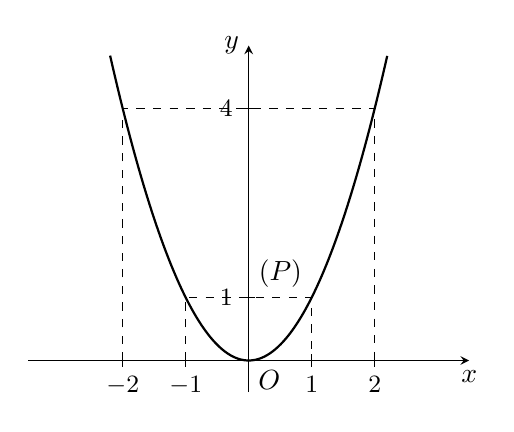
\begin{tikzpicture}[>=stealth,scale=0.8]
			\draw[->] (-3.5,0) -- (3.5,0) node[below] {$x$};
			\draw[->] (0,-0.5) -- (0,5) node[left] {$y$};
			\draw (0,0) node[below right] {$O$};
			\foreach \x in {-2,-1,1,2}
				\draw (\x,0.1) -- (\x,-0.1) node[below] {\small $\x$};
			\foreach \y in {1,4}
				\draw (0.1,\y) -- (-0.1,\y) node[left] {\small $\y$};
			\draw[dashed] (-1,0) -- (-1,1) -- (1,1) -- (1,0);
			\draw[dashed] (-2,0) -- (-2,4) -- (2,4) -- (2,0);
			\draw[thick,smooth,samples=100,domain=-2.2:2.2] plot(\x,{(\x)^2});
			\node[above left] at (1,1) {$(P)$};
		\end{tikzpicture}
	\end{center}
	\item Điểm $M$ thuộc $(P)$ có tung độ bằng hai lần hoành độ nên ta có $y = 2x$.\\
	Phương trình hoành độ giao điểm là:
	$$x^2 = 2x \iff x^2 - 2x = 0 \iff x(x - 2) = 0 \iff \left[\begin{aligned} &x = 0 \\ &x = 2. \end{aligned}\right.$$
	\begin{itemize}
		\item Với $x = 0 \implies y = 0$, ta được điểm $O(0; 0)$.
		\item Với $x = 2 \implies y = 2 \cdot 2 = 4$, ta được điểm $M(2; 4)$.
	\end{itemize}
	Vậy tọa độ các điểm cần tìm là $(0; 0)$ và $(2; 4)$.
\end{enumerate}
}
\end{bt}

\begin{bt}%[9D6H20-2]
% nguon: Đề tham khảo Tuyển sinh 10 năm học 2026-2027 Sở GD&ĐT TP.HCM - Cụm 5 Đề 2 - Bài 2
Cho phương trình bậc hai $3x^2 - 11x - 7 = 0$.
\begin{enumerate}[a)]
	\item Chứng minh phương trình luôn có hai nghiệm phân biệt $x_1, x_2$.
	\item Không giải phương trình, hãy tính giá trị của biểu thức:
	$$A = \left(\dfrac{1}{x_2} - \dfrac{1}{x_1}\right)(x_1 - x_2).$$
\end{enumerate}
\loigiai{
\begin{enumerate}[a)]
	\item Phương trình $3x^2 - 11x - 7 = 0$ có các hệ số $a = 3$, $b = -11$, $c = -7$.\\
	Ta có $a \cdot c = 3 \cdot (-7) = -21 < 0$.\\
	Vì $a$ và $c$ trái dấu nên phương trình luôn có hai nghiệm phân biệt $x_1, x_2$.
	\item Theo định lí Vi-ét, ta có:
	$$\left\{\begin{aligned} &x_1 + x_2 = -\dfrac{b}{a} = \dfrac{11}{3} \\ &x_1 x_2 = \dfrac{c}{a} = -\dfrac{7}{3}. \end{aligned}\right.$$
	Biến đổi biểu thức $A$:
	$$A = \left(\dfrac{1}{x_2} - \dfrac{1}{x_1}\right)(x_1 - x_2) = \dfrac{x_1 - x_2}{x_1 x_2}(x_1 - x_2) = \dfrac{(x_1 - x_2)^2}{x_1 x_2} = \dfrac{(x_1 + x_2)^2 - 4x_1 x_2}{x_1 x_2}.$$
	Thay các giá trị Vi-ét vào biểu thức $A$, ta được:
	$$A = \dfrac{\left(\dfrac{11}{3}\right)^2 - 4 \cdot \left(-\dfrac{7}{3}\right)}{-\dfrac{7}{3}} = \dfrac{\dfrac{121}{9} + \dfrac{28}{3}}{-\dfrac{7}{3}} = \dfrac{\dfrac{121 + 84}{9}}{-\dfrac{7}{3}} = \dfrac{\dfrac{205}{9}}{-\dfrac{7}{3}} = -\dfrac{205}{21}.$$
	Vậy $A = -\dfrac{205}{21}$.
\end{enumerate}
}
\end{bt}

\begin{bt}%[9D8H26-3]
% nguon: Đề tham khảo Tuyển sinh 10 năm học 2026-2027 Sở GD&ĐT TP.HCM - Cụm 5 Đề 2 - Bài 3
Bảng thống kê số lượng khách nội địa và khách quốc tế đến tham quan tại $6$ địa điểm của Việt Nam trong năm $2022$ (đơn vị: nghìn người):
\begin{center}
	\begin{tabular}{|l|c|c|c|c|c|c|}
		\hline
		\textbf{Địa điểm} & \textbf{Hạ Long} & \textbf{Đà Lạt} & \textbf{Nha Trang} & \textbf{Sapa} & \textbf{Phú Quốc} & \textbf{Đà Nẵng} \\ \hline
		\textbf{Khách nội địa} & $1200$ & $900$ & $1500$ & $720$ & $1300$ & $1800$ \\ \hline
		\textbf{Khách quốc tế} & $300$ & $100$ & $500$ & $80$ & $500$ & $1200$ \\ \hline
	\end{tabular}
\end{center}
\begin{enumerate}[a)]
	\item Hãy cho biết địa điểm nào có tỉ lệ khách quốc tế so với tổng số khách tham quan cao nhất và thấp nhất trong năm $2022$.
	\item Chọn ngẫu nhiên một địa điểm trong số $6$ địa điểm trên. Tính xác suất của các biến cố sau:
	\begin{itemize}
		\item $A$: ``Địa điểm được chọn có tổng số khách tham quan dưới $2000$ nghìn người''.
		\item $B$: ``Địa điểm được chọn có tỉ lệ khách quốc tế so với tổng số khách từ $20\%$ trở lên''.
	\end{itemize}
\end{enumerate}
\loigiai{
\begin{enumerate}[a)]
	\item Tỉ lệ khách quốc tế so với tổng số khách tại từng địa điểm là:
	\begin{itemize}
		\item Hạ Long: $\dfrac{300}{1200 + 300} = \dfrac{300}{1500} = 20\%$.
		\item Đà Lạt: $\dfrac{100}{900 + 100} = \dfrac{100}{1000} = 10\%$.
		\item Nha Trang: $\dfrac{500}{1500 + 500} = \dfrac{500}{2000} = 25\%$.
		\item Sapa: $\dfrac{80}{720 + 80} = \dfrac{80}{800} = 10\%$.
		\item Phú Quốc: $\dfrac{500}{1300 + 500} = \dfrac{500}{1800} \approx 27{,}78\%$.
		\item Đà Nẵng: $\dfrac{1200}{1800 + 1200} = \dfrac{1200}{3000} = 40\%$.
	\end{itemize}
	Vậy địa điểm có tỉ lệ khách quốc tế cao nhất là Đà Nẵng ($40\%$), thấp nhất là Đà Lạt và Sapa ($10\%$).
	\item Không gian mẫu có số phần tử là $n(\Omega) = 6$.
	\begin{itemize}
		\item Biến cố $A$: Các địa điểm có tổng số khách dưới $2000$ nghìn người là Hạ Long ($1500$), Đà Lạt ($1000$), Sapa ($800$), Phú Quốc ($1800$). Có $4$ địa điểm, nên $n(A) = 4$.\\
		Xác suất của biến cố $A$ là:
		$$P(A) = \dfrac{4}{6} = \dfrac{2}{3}.$$
		\item Biến cố $B$: Các địa điểm có tỉ lệ khách quốc tế từ $20\%$ trở lên là Hạ Long ($20\%$), Nha Trang ($25\%$), Phú Quốc ($\approx 27{,}78\%$), Đà Nẵng ($40\%$). Có $4$ địa điểm, nên $n(B) = 4$.\\
		Xác suất của biến cố $B$ là:
		$$P(B) = \dfrac{4}{6} = \dfrac{2}{3}.$$
	\end{itemize}
\end{enumerate}
}
\end{bt}

\begin{bt}%[9D6V21-3]
% nguon: Đề tham khảo Tuyển sinh 10 năm học 2026-2027 Sở GD&ĐT TP.HCM - Cụm 5 Đề 2 - Bài 4
Một khu vườn hình bán nguyệt $SRT$ có tâm $O$ và bán kính $R = 12\text{ m}$. Một khu vực trồng cỏ hình quạt tròn $PQR$ có tâm $Q$, bán kính $QP = QR = 16\text{ m}$ và $O$ là trung điểm của đoạn thẳng $PQ$. Chiều dài cung tròn $PR$ là $14\text{ m}$. Phần diện tích còn lại của khu vườn bán nguyệt được rào lại để trồng hoa.
\begin{enumerate}[a)]
	\item Tính chiều dài hàng rào bao quanh khu vực trồng hoa theo số $\pi$.
	\item Tính diện tích khu vực trồng hoa (kết quả làm tròn đến hàng phần mười).
\end{enumerate}
\loigiai{
\begin{enumerate}[a)]
	\item Vì $O$ là trung điểm của $PQ$ nên $OP = OQ = \dfrac{QP}{2} = \dfrac{16}{2} = 8\text{ (m)}$.\\
	Bán kính của hình bán nguyệt tâm $O$ là $OS = OT = 12\text{ m}$, do đó:
	$$SP = OS - OP = 12 - 8 = 4\text{ (m)}, \quad QT = OT - OQ = 12 - 8 = 4\text{ (m)}.$$
	Hàng rào bao quanh khu vực trồng hoa gồm: cung bán nguyệt $SRT$, đoạn thẳng $SP$, đoạn thẳng $QT$, cung tròn $PR$ và bán kính $QR$.\\
	Chiều dài cung bán nguyệt $SRT$ là: $\pi R = 12\pi\text{ (m)}$.\\
	Tổng chiều dài hàng rào là:
	$$L = 12\pi + SP + QT + \text{cung } PR + QR = 12\pi + 4 + 4 + 14 + 16 = 12\pi + 38\text{ (m)}.$$
	\item Diện tích hình bán nguyệt tâm $O$, bán kính $R = 12\text{ m}$ là:
	$$S_{\text{bn}} = \dfrac{1}{2}\pi R^2 = \dfrac{1}{2}\pi \cdot 12^2 = 72\pi\text{ (m}^2\text{)}.$$
	Diện tích khu vực trồng cỏ (hình quạt tròn tâm $Q$, bán kính $r = 16\text{ m}$, độ dài cung $l = 14\text{ m}$) là:
	$$S_{\text{cỏ}} = \dfrac{1}{2} r \cdot l = \dfrac{1}{2} \cdot 16 \cdot 14 = 112\text{ (m}^2\text{)}.$$
	Diện tích khu vực trồng hoa là:
	$$S_{\text{hoa}} = S_{\text{bn}} - S_{\text{cỏ}} = 72\pi - 112 \approx 72 \cdot 3{,}14159 - 112 \approx 226{,}2 - 112 = 114{,}2\text{ (m}^2\text{)}.$$
	Vậy diện tích khu vực trồng hoa là khoảng $114{,}2\text{ m}^2$.
\end{enumerate}
}
\end{bt}

\begin{bt}%[9H0V31-3]
% nguon: Đề tham khảo Tuyển sinh 10 năm học 2026-2027 Sở GD&ĐT TP.HCM - Cụm 5 Đề 2 - Bài 5
Một loại cam sành dạng hình cầu có đường kính $8\text{ cm}$, vỏ cam dày $0{,}3\text{ cm}$. Coi phần ruột quả cam cũng có dạng hình cầu đồng tâm với quả cam và mỗi quả khi ép lấy nước thu được lượng nước cam bằng $88\%$ thể tích phần ruột. Lấy $\pi \approx 3{,}14$.
\begin{enumerate}[a)]
	\item Tính thể tích phần ruột của một quả cam (kết quả làm tròn đến hàng phần trăm).
	\item Một quán giải khát pha nước cam bằng cách trộn nước ép cam nguyên chất với nước lọc theo tỉ lệ $3 : 1$ (theo thể tích). Hỏi quán cần dùng ít nhất bao nhiêu quả cam như trên để pha được $5$ lít nước cam thành phẩm theo tỉ lệ đó?
\end{enumerate}
\loigiai{
\begin{enumerate}[a)]
	\item Bán kính của quả cam là $R = \dfrac{8}{2} = 4\text{ (cm)}$.\\
	Vì vỏ cam dày $0{,}3\text{ cm}$ nên bán kính phần ruột của quả cam là:
	$$r = R - 0{,}3 = 4 - 0{,}3 = 3{,}7\text{ (cm)}.$$
	Thể tích phần ruột của một quả cam là:
	$$V_{\text{ruột}} = \dfrac{4}{3}\pi r^3 \approx \dfrac{4}{3} \cdot 3{,}14 \cdot (3{,}7)^3 = \dfrac{4}{3} \cdot 3{,}14 \cdot 50{,}653 \approx 212{,}07\text{ (cm}^3\text{)}.$$
	\item Đổi $5\text{ lít} = 5000\text{ cm}^3$.\\
	Nước cam thành phẩm được pha từ nước ép cam nguyên chất và nước lọc theo tỉ lệ thể tích là $3 : 1$ (gồm $3 + 1 = 4$ phần bằng nhau).\\
	Thể tích nước ép cam nguyên chất cần có trong $5$ lít nước cam thành phẩm là:
	$$V_{\text{nguyên chất}} = \dfrac{3}{4} \cdot 5000 = 3750\text{ (cm}^3\text{)}.$$
	Lượng nước ép thu được từ mỗi quả cam là:
	$$V_{\text{ép}} = 88\% \cdot V_{\text{ruột}} \approx 0{,}88 \cdot 212{,}07 \approx 186{,}62\text{ (cm}^3\text{)}.$$
	Số quả cam cần dùng là:
	$$n = \dfrac{V_{\text{nguyên chất}}}{V_{\text{ép}}} \approx \dfrac{3750}{186{,}62} \approx 20{,}09\text{ (quả)}.$$
	Vì số quả cam phải là số nguyên dương và nếu chỉ dùng $20$ quả thì chưa đủ lượng nước ép cần thiết ($20 \cdot 186{,}62 = 3732{,}4\text{ cm}^3 < 3750\text{ cm}^3$), nên quán cần dùng ít nhất $21$ quả cam.
\end{enumerate}
}
\end{bt}

\begin{bt}%[9D1H3-4]
% nguon: Đề tham khảo Tuyển sinh 10 năm học 2026-2027 Sở GD&ĐT TP.HCM - Cụm 5 Đề 2 - Bài 6
Trong một giải đấu cờ vua có $5$ vận động viên thi đấu vòng tròn một lượt (mỗi vận động viên đấu đúng một trận với $4$ vận động viên còn lại). Cách tính điểm: mỗi trận thắng được $1{,}0$ điểm, mỗi trận hòa được $0{,}5$ điểm, trận thua không có điểm. Sau khi kết thúc giải đấu, cả $5$ vận động viên đều có điểm số khác nhau và được xếp hạng lần lượt từ nhất đến năm. Biết rằng:
\begin{itemize}
	\item Vận động viên xếp hạng nhất không hòa trận nào;
	\item Vận động viên xếp hạng nhì không thua trận nào;
	\item Vận động viên xếp hạng tư không thắng trận nào.
\end{itemize}
\begin{enumerate}[a)]
	\item Giải đấu đã tổ chức tất cả bao nhiêu trận đấu và vận động viên xếp hạng nhất đạt được bao nhiêu điểm?
	\item Hãy xác định điểm số của mỗi vận động viên còn lại và chi tiết kết quả các trận đấu của từng vận động viên.
\end{enumerate}
\loigiai{
\begin{enumerate}[a)]
	\item Số trận đấu của giải là:
	$$\dfrac{5 \cdot 4}{2} = 10\text{ (trận)}.$$
	Vì mỗi trận đấu luôn mang lại tổng cộng $1$ điểm cho cả hai đấu thủ (thắng nhận $1$ và thua nhận $0$, hoặc mỗi người nhận $0{,}5$ khi hòa), nên tổng số điểm của cả giải đấu là $10 \cdot 1 = 10$ điểm.\\
	Gọi số điểm của $5$ vận động viên xếp hạng từ nhất đến năm lần lượt là $A_1 > A_2 > A_3 > A_4 > A_5$.\\
	Ta có $A_1 + A_2 + A_3 + A_4 + A_5 = 10$.\\
	Vì vận động viên hạng nhất không hòa trận nào nên số điểm $A_1$ phải là số nguyên.\\
	Vận động viên hạng nhì không thua trận nào, nên trong trận đối đầu trực tiếp giữa hạng nhất và hạng nhì: vận động viên hạng nhì không thể thua và vận động viên hạng nhất không thể hòa, do đó vận động viên hạng nhì phải thắng vận động viên hạng nhất.\\
	Điều này có nghĩa vận động viên hạng nhất thua ít nhất $1$ trận, suy ra số trận thắng tối đa của vận động viên hạng nhất là $3$ trận.\\
	Do đó vận động viên hạng nhất đạt được $3$ điểm ($3$ thắng, $1$ thua).
	\item Vì $A_1 = 3$, nên tổng số điểm của $4$ vận động viên còn lại là:
	$$A_2 + A_3 + A_4 + A_5 = 10 - 3 = 7\text{ (điểm)}.$$
	Điểm số của các vận động viên phải là bội số của $0{,}5$ và thỏa mãn $3 > A_2 > A_3 > A_4 > A_5$.\\
	Bộ số thỏa mãn điều kiện thứ tự giảm dần và có tổng bằng $7$ là:
	$$A_2 = 2{,}5; \quad A_3 = 2{,}0; \quad A_4 = 1{,}5; \quad A_5 = 1{,}0.$$
	Kiểm tra tính hợp lí của kết quả thi đấu:
	\begin{itemize}
		\item VĐV hạng nhì đạt $2{,}5$ điểm: Thắng VĐV nhất ($1$ điểm), hòa cả $3$ VĐV còn lại ($3 \cdot 0{,}5 = 1{,}5$ điểm) $\implies$ không thua trận nào (thỏa mãn).
		\item VĐV hạng tư đạt $1{,}5$ điểm: VĐV hạng tư không thắng trận nào, thua VĐV nhất và hòa cả $3$ VĐV còn lại ($3 \cdot 0{,}5 = 1{,}5$ điểm) $\implies$ thỏa mãn.
		\item VĐV hạng ba đạt $2{,}0$ điểm: Thua VĐV nhất ($0$ điểm), hòa VĐV nhì ($0{,}5$ điểm), hòa VĐV tư ($0{,}5$ điểm), thắng VĐV năm ($1$ điểm) $\implies$ tổng $2{,}0$ điểm (thỏa mãn).
		\item VĐV hạng năm đạt $1{,}0$ điểm: Thua VĐV nhất và VĐV ba, hòa VĐV nhì và VĐV tư ($2 \cdot 0{,}5 = 1$ điểm) $\implies$ thỏa mãn.
	\end{itemize}
	Vậy điểm số cụ thể của các vận động viên là: hạng nhì được $2{,}5$ điểm; hạng ba được $2{,}0$ điểm; hạng tư được $1{,}5$ điểm; hạng năm được $1{,}0$ điểm.
\end{enumerate}
}
\end{bt}

\begin{bt}%[9H9C29-3]
% nguon: Đề tham khảo Tuyển sinh 10 năm học 2026-2027 Sở GD&ĐT TP.HCM - Cụm 5 Đề 2 - Bài 7
Từ điểm $A$ nằm ngoài đường tròn $(O; R)$, vẽ tiếp tuyến $AB$ với đường tròn ($B$ là tiếp điểm) và đường kính $BC$. Đoạn thẳng $AC$ cắt đường tròn $(O)$ tại điểm $D$ ($D$ khác $C$). Kẻ $BH \perp AO$ tại $H$.
\begin{enumerate}[a)]
	\item Chứng minh $BD \perp AC$ tại $D$ và bốn điểm $A, B, H, D$ cùng thuộc một đường tròn.
	\item Chứng minh $OB^2 = OH \cdot OA$ và $\widehat{OHC} = \widehat{AHD}$.
	\item Khi $AH = 12\text{ cm}$ và $OH = 9\text{ cm}$, hãy tính diện tích hình viên phân giới hạn bởi cung nhỏ $BD$ và dây cung $BD$ (kết quả làm tròn đến chữ số thập phân thứ hai).
\end{enumerate}
\loigiai{
\begin{center}
	\begin{tikzpicture}[scale=0.9,>=stealth]
		\coordinate (O) at (0,0);
		\def\R{2.8}
		\draw[thick] (O) circle (\R);
		\coordinate (B) at (-\R,0);
		\coordinate (C) at (\R,0);
		% Tiep tuyen tai B thang dung: x = -R
		% Cho A co toa do (-R, 4.2)
		\coordinate (A) at (-\R,3.8);
		\coordinate (H) at ($(A)!(B)!(O)$);
		% Giao diem D cua AC voi (O)
		\path [name path=circle] (O) circle (\R);
		\path [name path=AC] (A) -- (C);
		\coordinate (D) at (0.97,2.62);

		\draw[thick] (B) -- (C);
		\draw[thick] (A) -- (B);
		\draw[thick] (A) -- (C);
		\draw[thick] (B) -- (D);
		\draw[thick] (A) -- (O);
		\draw[thick] (B) -- (H);
		\draw[dashed] (O) -- (D);
		\draw[dashed] (H) -- (C);
		\draw[dashed] (H) -- (D);

		\fill (O) circle (1.5pt) node[below] {$O$};
		\fill (B) circle (1.5pt) node[left] {$B$};
		\fill (C) circle (1.5pt) node[right] {$C$};
		\fill (A) circle (1.5pt) node[above left] {$A$};
		\fill (H) circle (1.5pt) node[above right] {$H$};
		\fill (D) circle (1.5pt) node[above] {$D$};
	\end{tikzpicture}
\end{center}
\begin{enumerate}[a)]
	\item Ta có $\widehat{BDC} = 90^\circ$ (góc nội tiếp chắn nửa đường tròn đường kính $BC$).\\
	Suy ra $BD \perp AC$ tại $D$.\\
	Xét tứ giác $ABHD$:
	\begin{itemize}
		\item Vì $BH \perp AO$ tại $H$ nên $\widehat{AHB} = 90^\circ$, do đó tam giác $ABH$ vuông tại $H$ nội tiếp đường tròn đường kính $AB$;
		\item Vì $BD \perp AC$ tại $D$ nên $\widehat{ADB} = 90^\circ$, do đó tam giác $ADB$ vuông tại $D$ nội tiếp đường tròn đường kính $AB$.
	\end{itemize}
	Vậy bốn điểm $A, B, H, D$ cùng thuộc đường tròn đường kính $AB$.
	\item Vì $AB$ là tiếp tuyến tại $B$ của $(O)$ nên $AB \perp OB$ tại $B$.\\
	Tam giác $ABO$ vuông tại $B$ có đường cao $BH$ ($BH \perp AO$), áp dụng hệ thức lượng ta có:
	$$OB^2 = OH \cdot OA.$$
	Vì $OB = OC = R$ nên $OC^2 = OH \cdot OA \implies \dfrac{OH}{OC} = \dfrac{OC}{OA}$.\\
	Xét $\Delta OHC$ và $\Delta OCA$ có:
	\begin{itemize}
		\item Góc $\widehat{COA}$ chung;
		\item $\dfrac{OH}{OC} = \dfrac{OC}{OA}$.
	\end{itemize}
	Do đó $\Delta OHC \backsim \Delta OCA$ (c-g-c) $\implies \widehat{OHC} = \widehat{OCA}$ (1).\\
	Trong tam giác vuông $ABC$ (vuông tại $B$): $\widehat{OCA} = \widehat{BCA} = 90^\circ - \widehat{BAC} = \widehat{ABD}$ (2).\\
	Mặt khác, tứ giác $ABHD$ nội tiếp nên $\widehat{ABD} = \widehat{AHD}$ (hai góc nội tiếp cùng chắn cung $AD$) (3).\\
	Từ (1), (2) và (3) suy ra $\widehat{OHC} = \widehat{AHD}$.
	\item Khi $AH = 12\text{ cm}$ và $OH = 9\text{ cm}$, ta có:
	$$OA = AH + OH = 12 + 9 = 21\text{ (cm)}.$$
	Theo câu b:
	$$R^2 = OB^2 = OH \cdot OA = 9 \cdot 21 = 189 \implies R = \sqrt{189} = 3\sqrt{21}\text{ (cm)}.$$
	Tam giác $ABO$ vuông tại $B$ có:
	$$AB = \sqrt{OA^2 - OB^2} = \sqrt{21^2 - 189} = \sqrt{441 - 189} = \sqrt{252} = 6\sqrt{7}\text{ (cm)}.$$
	Tam giác $ABC$ vuông tại $B$ có đường cao $BD$:
	$$BD = \dfrac{AB \cdot BC}{AC} = \dfrac{AB \cdot 2R}{\sqrt{AB^2 + (2R)^2}} = \dfrac{6\sqrt{7} \cdot 6\sqrt{21}}{\sqrt{252 + 756}} = \dfrac{252\sqrt{3}}{\sqrt{1008}} = \dfrac{252\sqrt{3}}{12\sqrt{7}} = 3\sqrt{21}\text{ (cm)}.$$
	Nhận thấy $BD = OB = OD = R = 3\sqrt{21}\text{ cm}$, do đó tam giác $OBD$ là tam giác đều.\\
	Suy ra góc ở tâm $\widehat{BOD} = 60^\circ$.\\
	Diện tích hình quạt tròn giới hạn bởi cung nhỏ $BD$ là:
	$$S_q = \dfrac{\pi R^2 \cdot 60^\circ}{360^\circ} = \dfrac{\pi \cdot 189}{6} = \dfrac{63\pi}{2} \approx 98{,}96\text{ (cm}^2\text{)}.$$
	Diện tích tam giác đều $OBD$ là:
	$$S_{\Delta OBD} = \dfrac{R^2\sqrt{3}}{4} = \dfrac{189\sqrt{3}}{4} \approx 81{,}84\text{ (cm}^2\text{)}.$$
	Diện tích hình viên phân cần tìm là:
	$$S = S_q - S_{\Delta OBD} \approx 98{,}96 - 81{,}84 = 17{,}12\text{ (cm}^2\text{)}.$$
	Vậy diện tích hình viên phân là $17{,}12\text{ cm}^2$.
\end{enumerate}
}
\end{bt}
